\documentclass[journal,10pt,twocolumn]{article}
\usepackage{graphicx}
\usepackage[margin=0.5in]{geometry}
\usepackage[cmex10]{amsmath}
\usepackage{array}
\usepackage{booktabs}
\title{\textbf{Line Assignment}}
\author{Hari Venkateswarlu}
\date{September 2022}

\providecommand{\norm}[1]{\left\lVert#1\right\rVert}
\providecommand{\abs}[1]{\left\vert#1\right\vert}
\let\vec\mathbf
\newcommand{\myvec}[1]{\ensuremath{\begin{pmatrix}#1\end{pmatrix}}}
\newcommand{\mydet}[1]{\ensuremath{\begin{vmatrix}#1\end{vmatrix}}}
\providecommand{\brak}[1]{\ensuremath{\left(#1\right)}}

\begin{document}

\maketitle
\paragraph{\textit{Problem Statement} - Find a point on the x-axis,which is equidistant from the points$\begin{pmatrix}
  7 \\
  6 \\
 \end{pmatrix}$ and $\begin{pmatrix}
  3 \\
  4 \\
 \end{pmatrix}$}
\begin{enumerate}
\item finding the point on x-axis which is equidistant from the points
\end{enumerate}

\begin{figure}[h]
\centering
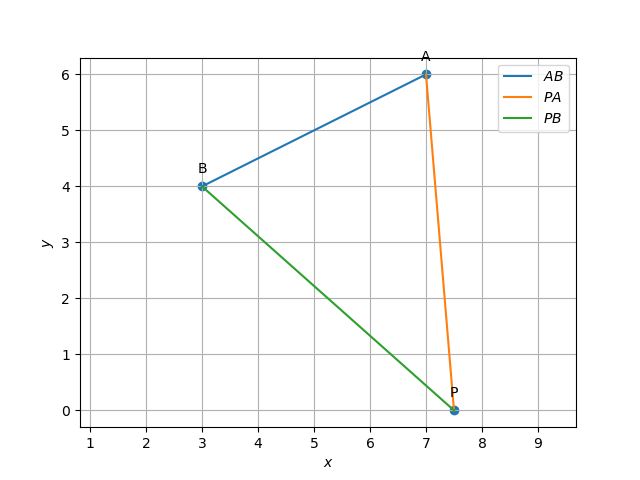
\includegraphics[width=1\columnwidth]{Figure1.png}

\label{fig}
\end{figure}

\section*{Solution}
Given points
A=$\begin{pmatrix}
  7 \\
  6 \\
 \end{pmatrix}$
 and B=$\begin{pmatrix}
  3 \\
  4 \\
 \end{pmatrix}$


if the point is lying on x-axis then y-axis will be zero i.e.. y=0


Distance between the points $\begin{pmatrix}
  7 \\
  6 \\
 \end{pmatrix}$ and $\begin{pmatrix}
  x \\
  0 \\
 \end{pmatrix}$= Distance between the points $\begin{pmatrix}
  3 \\
  4 \\
 \end{pmatrix}$ and $\begin{pmatrix}
  x \\
  0 \\
 \end{pmatrix}$\\ 	     

Consider P on x-axis P$\begin{pmatrix}
  x \\
  0 \\
 \end{pmatrix}$           \vspace{3mm}

	$|AP|$=$|BP|$\\   \vspace{3mm}
A$\begin{pmatrix}
  7 \\
  6 \\
 \end{pmatrix}$$|A_0|$=$\sqrt{(7-x)^2+(6-0)^2}$\\     \vspace{3mm}
B$\begin{pmatrix}
  3 \\
  4 \\
 \end{pmatrix}$ $|B_0|$=$\sqrt{(3-x)^2+(4-0)^2}$\\      \vspace{3mm}
$|A_0|$=$|B_0|$\\             \vspace{2mm}                 
$(7-x)^2+36=(3-x)^2+16$\\      \vspace{2mm}                
$(7-x)^2+20=(3-x)^2$\\           \vspace{2mm}              
$49+x^2-14x+20=9+x^2-6x$\\         \vspace{2mm}            
$60=8x$\\                            \vspace{2mm}          
$x=60/8$\\                           \vspace{2mm}          
$x=7.5$                  			
\end{document}
